
\section{Introduction}
% \ha{consider to structure as introduction format in Computer Science, you can consider to refer the introductio of this paper: \url{https://www.csie.ntu.edu.tw/~htlin/paper/doc/pakdd25aclimage.pdf}}
Imbalanced learning refers to scenarios where certain classes are significantly underrepresented compared to others in a dataset \cite{cao2019learning, cheng2023smote, vu2024lcsl, mai2025-icm, prototype-longtailed}.
This disparity can severely impact the performance of machine learning models, as they often become biased towards the majority class, leading to suboptimal predictions for the minority class. Such challenges are especially prevalent in critical domains like medical diagnosis, fraud detection, and rare event forecasting, where identifying the minority class accurately is of utmost importance \cite{krawczyk2016learning, he2009learning, le2024semantic}.

\begin{figure}[t]
    \centering
        \centering
        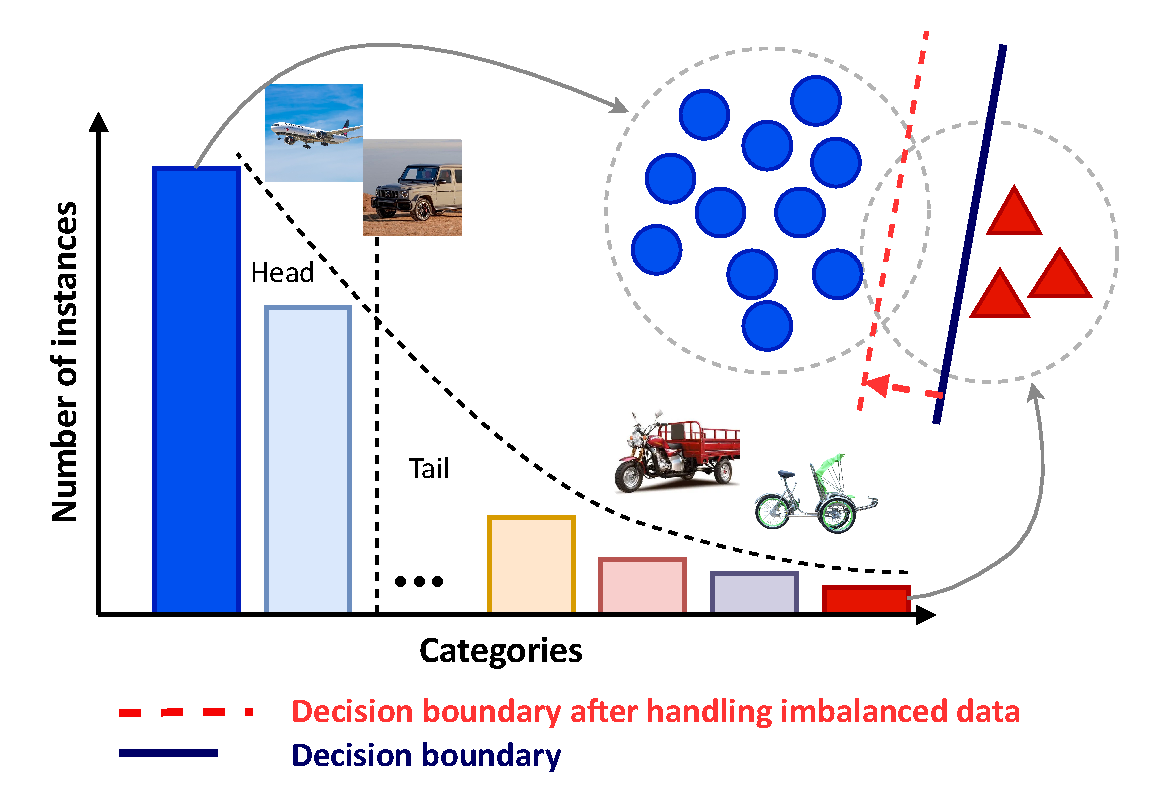
\includegraphics[width=\columnwidth]{imbalance-Page-2.drawio.pdf}
        \caption{Visualization of a long-tailed dataset distribution. The graph illustrates that certain categories, like airplanes and trucks, appear frequently in the dataset, while other less common or specialized vehicles, such as three-wheeled motorbike, occur much less often. This long-tailed distribution reflects real-world imbalances where some classes dominate, and many others have sparse representation.}
\label{fig:cifar10_imbalance_combined}
\end{figure}

Addressing imbalanced data requires strategies that can mitigate the inherent difficulties posed by skewed distributions. Traditional approaches fall broadly into three categories: data-level techniques, algorithm-level modifications, and hybrid methods \cite{sun2009classification, he2009learning}. Data-level techniques, such as oversampling and undersampling~\cite{unbiased_sample}, adjust the distribution by replicating minority class samples or reducing majority class samples. Algorithmic modifications, such as cost-sensitive learning, assign higher misclassification penalties to the minority class, thereby improving its representation during training. Hybrid approaches combine these strategies for enhanced performance. Prominent examples include Synthetic Minority Over-sampling Technique (SMOTE), ensemble-based methods, and cost-sensitive learning frameworks \cite{chawla2002smote, he2009learning}.

Recent advancements, such as  Margin-Aware Mixup (MAMix), have introduced Mixup-based data augmentation and adaptive learning strategies, significantly improving model generalization on imbalanced datasets \cite{cheng2023smote}. MAMix enhances minority class representations and mitigates decision boundary bias by dynamically adjusting Mixup parameters during training. Despite these developments, deep learning models remain vulnerable to class imbalance due to their dependency on large datasets and their tendency to amplify biases towards the majority class \cite{krawczyk2016learning}. This vulnerability underscores the need for more effective and computationally efficient solutions.
\textbf{Motivation.} While numerous techniques exist to address imbalanced learning, many involve a trade-off between computational efficiency, scalability, and model accuracy. Traditional resampling methods often require extensive parameter tuning and can be computationally intensive \cite{he2009learning}.
%Recent state-of-the-art methods such as Generative Adversarial Networks (GANs) have shown remarkable versatility and effectiveness in imbalanced learning \cite{yadav2025rebalancingscalessystematicmapping}, but they also face several long-standing challenges and limitations, such as excessive resource utilization and implementation constraints.
The field is bounded by resource-intensive deep learning on the end and less effective tuning-heavy traditional methods on the other. Between these two extremes lie the lightweight imbalanced learning techniques. They minimize computational overhead without sacrificing performance and are becoming increasingly critical, especially in resource-constrained environments such as Internet of Things (IoT) and edge devices.
%Techniques such as Mixup \cite{zhang2017Mixup}, when combined with Deferred Re-Weighting (DRW) schedules \cite{cao2019learning}, present promising alternatives by more effectively distributing the data during training and maintaining.
% \textbf{Fair Comparison and Lightweight Techniques.} To evaluate the effectiveness of lightweight strategies and sampling methods, it is essential to systematically analyze their impact on both computational efficiency and model performance. This involves considering trade-offs in time complexity, scalability, and classification accuracy. Such an analysis is particularly relevant for deep learning, where the issue of class imbalance is often magnified.
\texorpdfstring{\textbf{Objective.}}{Objective.}
Our objective is to identify
the most suitable augmentation approach for each specific
method, avoiding the extremes of underutilization and overutilization in ways that might introduce noise or degrade model performance. By systematically analyzing augmentation placement within the training pipeline, our objective is to develop a highly adaptive, context-aware augmentation strategy. The goal is to maximize generalization and performance in diverse machine learning applications.

\textbf{Contribution.} 
In this work, we focus on lightweight approaches to resolving class imbalance, with an emphasis on integrating Mixup with DRW schedules. By systematically comparing these methods across various resampling strategies, we demonstrate that combining Mixup and DRW achieves significant improvements in model performance while keeping the computational cost under control. This study contributes to advancing the state-of-the-art by providing scalable, robust solutions for imbalanced learning scenarios, where computing resources are under constraint. Moreover, we further investigate to determine the optimal timing and conditions for applying augmentation techniques. Understanding when and how to introduce data augmentation is crucial, as different augmentation strategies may yield varying levels of effectiveness depending on the dataset characteristics, model architecture, and training dynamics.

The remainder of this paper is organized as follows. Section~\ref{sec:related_work} reviews prior work in the field. In Section~\ref{sec:motivation}, we present the motivation for adopting lightweight techniques. Our proposed methodology is detailed in Section~\ref{sec:methodology}. We describe our experimental setup in Section~\ref{sec:experiments}, present our main results and a detailed ablation study in Section~\ref{sec:ablation}, and conclude in Section~\ref{sec:conclusion}.